\documentclass[a4paper,10pt]{article}
\usepackage{a4wide}
\usepackage{caratula}
\usepackage[pdftex]{graphicx}
\usepackage[spanish]{babel}
\usepackage[latin1]{inputenc}
\usepackage{listings}
\usepackage{makeidx} 
\makeindex

\newcommand{\fileh}[1]{\noindent\textsf{Archivo: }\texttt{#1} \hfill\ }
\newcommand{\jc}[1]{\texttt{#1}} % TODO make ref

\begin{document}

\titulo{Noam}
\subtitulo{Conversiones entre formalismos de lenguajes}
\fecha{17 de Julio de 2008}
\materia{Teor�a de Lenguajes}
\integrante{Cardiff, Brian Jonathan}{784/03}{bcardiff@gmail.com}
\integrante{Savoretti, Sonia Florencia}{785/03}{soniaflorencia@gmail.com}
\integrante{Geier, Maximiliano Iv�n}{477/04}{migeier@gmail.com}

\maketitle

\tableofcontents

\section{Conversiones entre formalismos}

El siguiente gr�fico muestra los algoritmos implementados para convertir de un 
formalismo a otro. 

\begin{center}
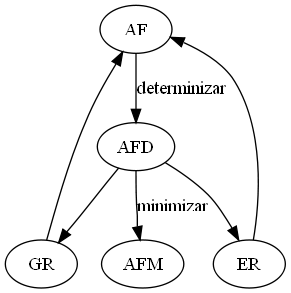
\includegraphics[width=7cm]{conversiones.png}
\end{center}

Luego, por ejemplo para convertir de ER a AFM se realizan las conversiones
intermedias a AF y a AFD. En el caso de AFM a AFD o AF no se realiza conversi�n alguna, 
as� como tampoco para AFD a AF.

A continuaci�n se hacen comentarios sobre los distintos algoritmos de conversi�n.

\subsection{AF a AFD. Determinizar}

Se aplica directamente la eliminaci�n de transiciones lambda y la determinizaci�n
del aut�mata. Se implementa en \jc{Determination}.

\subsection{AFD a AFM. Minimizar}

Luego de completar el AFD usando \jc{Complete} y eliminar los estados no alcanzables usando
\jc{Reachables}, se aplica el algoritmo de minimizaci�n visto en clase e implementado en \jc{Minimization}.

Como resultado de la minimizaci�n es posible que se generen aut�matas sin estados finales. 
Elegimos contemplar la generaci�n de los aut�matas sin estados finales, por m�s que no
sean parte de la gram�tica. Claramente �sto se presenta cuando el lenguaje que se describe
es $\emptyset$ ej.:  VACIO, VACIO.a.

\subsection{AFD a ER}

Se implementa el algoritmo recursivo que plantea $R^k_{ij}$ como el lenguaje regular que se
obtiene desde el estado $s_i$ al estado $s_j$ pasando a lo sumo por $s_1, \ldots, s_k$ como estados intermedios.

La implementaci�n se encuentra en \jc{AFDtoER}.

\subsection{ER a AF}

Se hace una transformaci�n recursiva en la estructura de la ER basada en la demostraci�n
de inclusi�n de lenguajes aceptados por expresiones regulares en los aceptados 
por aut�matas finitos del Hopcroft et.al..

La �nica diferencia es el caso de la clausura. En lugar de agregar un estado final y uno inicial, se preserva
el estado inicial, se agregan transiciones lambda desde todos los finales al inicial, y se define al estado inicial
como �nico estado final.

La implementaci�n se encuentra en \jc{ERToAutomata}.

\subsection{AFD a GR}

TODO

\subsection{GR a AF}

Como las gram�ticas tratadas son recursivas simples a derecha la transformaci�n se pone
un estado $q_A$ por cada s�mbolo no terminal $A$, el estado inicial se corresponde con el 
s�mbolo distinguido y cada producci�n se traduce como sigue:

\begin{description}
\item[$A \rightarrow \lambda$] se agrega el estado $q_A$ como estado final.
\item[$A \rightarrow tB$] se agrega una transici�n con label $t$ desde $q_A$ hacia $q_B$.
\item[$A \rightarrow t$] se agrega a una ... TODO ...
\end{description}

\section{TODO}

Para los casos de formalismos de entrada AFD y AFM, se toma como v�lido la entrada si corresponde exactamente con dicho formalismo.

Simplificaciones en la conversion de ER a AF

Descripci�n de las conversiones. hacer tablita.
\section{Ejemplos}

\section{Desarrollo}

El desarrollo del proyecto se realiz� con Eclipse 3.2. Se usaron las siguientes bibliotecas y plug-ins de eclipse:

\begin{description}
\item[antlr-eclipse] \verb"http://antlreclipse.sourceforge.net/" plug-in de eclipse con soporte para
edici�n y compilaci�n integrada de gram�ticas AntLR 2.7.6 .
\item[JUnit4]
\item[java-getopt] biblioteca incluida en \verb"/lib" para el tratamiento de argumentos por l�nea de comandos.
\item[FatJar] \verb"http://fjep.sourceforge.net/" plug-in de eclipse para generar un jar sin dependencias.
\end{description}

Dado que se us� FatJar, para usar la aplicaci�n lo �nico necesario es ejecutar

\begin{verbatim}
#> java -jar noam.jar -i <GR|ER|AF|AFD|AFM> [-o <GR|ER|AF|AFD|AFM>]
\end{verbatim}

\section{Descripci�n por package}
\subsection{package noam}

Se encuentra el punto de entrada (\jc{EntryPoint}), funcionalidad auxiliar de entrada/salida (\jc{IO}), y conversores de formalismos (\jc{FormalismConverter} y descendientes).

Hay un \jc{FormalismConverter} por formalismo que identifica el formalismo inicial. �stos se encargan de validar la entrada y realizar la conversi�n hacia los otros formalismos.
La clase abstracta \jc{FormalismConverter} define c�mo obtener un AFD y un AFM a partir de un AF. Luego, en las clases descendientes solo es necesario definir la conversi�n a AF.

\subsection{package noam.af}

Se encuentra la representaci�n de un AF (cualquier aut�mata finito). Un AF es todo aquel que implementa la interfaz \jc{AF}.
Hay una implementaci�n trivial: \jc{AFND}.

Tambi�n se encuentra la interfaz \jc{IAutomataBuilder} que es usada para desacoplar la creaci�n de un aut�mata de la clase que lo representa. �sto se usa en el parser.

\subsection{package noam.af.algorithms}

Se encuentran los algoritmos de conversi�n de AF hacia ER y a GR; y los algoritmos de manipulaci�n de aut�matas.

Los algoritmos de manipulaci�n de aut�matas se implementan usando el patr�n \emph{Decorator}. En algunos algoritmos es necesario
crear estados nuevos, para simplificar el desarrollo de los mismo, los aut�matas (pero no el parser) soportan estados con nombres de m�s
de una letra. Como �ltima etapa en la conversi�n (\jc{FormalismConverter}) se aplica un renombre de estados usando los nombres: A, B, $\ldots$, Z, AA, AB, $\ldots$ en
un mejor esfuerzo por obtener un aut�mata v�lido para la gram�tica.

\subsection{package noam.af.grammar}

Se encuentra la gram�tica de AF y las clases generadas por AntLR a partir de �sta.

La gram�tica utiliza como contexto de ejecuci�n un \jc{IAutomataBuilder}, llamando a los 
m�todos que correspondan de acuerdo a lo que se est� parseando ej.: agregado de estados, terminales, transiciones, etc. 

\subsection{package noam.af.internal}

Se encuentra implentaci�n de \jc{IAutomataBuilder} que genera un \jc{AFND}.

\subsection{package noam.er}

Se encuentra clases de representaci�n del AST de expresiones regulares. La jerarqu�a empieza en \jc{ER}.
Se implementa el patr�n \emph{Visitor} por medio de \jc{IVisitor}.

\subsection{package noam.er.algorithms}

Se encuentran algoritmos para conversi�n de ER a AF y para la impresi�n de una ER, los mismos se implementan usando el patr�n \emph{Visitor}.

\subsection{package noam.er.grammar}

Se encuentra la gram�tica de ER y las clases generadas por AntLR a partir de �sta.

Cada regla de la gram�tica retorna una instancia que representa el AST generado por dicha regla.

\subsection{package noam.gr}

Se encuentra la representaci�n de una gram�tica (\jc{Grammar}). 

Tambi�n se encuentra la interfaz \jc{IGrammarBuilder} que es usada para desacoplar la creaci�n de una gram�tica del parser.

\subsection{package noam.gr.algorithms}

Se encuentra la conversi�n de GR a AF y un algoritmo para normalizaci�n de gram�ticas para asegurar que solo aparezcan producciones lambda para el s�mbolo distinguido.

\subsection{package noam.gr.grammar}

Se encuentra la gram�tica de GR y las clases generadas por AntLR a partir de �sta.

La gram�tica utiliza como contexto de ejecuci�n un \jc{IGrammarBuilder}, llamando a los 
m�todos que corresponda de acuerdo a lo que se est� parseando ej.: agregado de no terminales, terminales, producciones, etc. 

\subsection{package noam.gr.internal}

Se encuentra una implentaci�n de \jc{IGrammarBuilder} que genera un \jc{Grammar}.

\subsection{package noam.utils}

Se encuentran funciones auxiliares de uso general. Entre otras para la manipulaci�n de iteradores con fluidez.

\section{C�digo fuente AntLR}
\lstset{numbers=left, frame=single, tabsize=2, breaklines=true}
\subsection{package noam.af.grammar}

\fileh{noam/af/grammar/AfGrammar.g}
\index{grammar!AfGrammar}
\lstinputlisting{../src/noam/af/grammar/AfGrammar.g}

\subsection{package noam.er.grammar}

\fileh{noam/er/grammar/ERGrammar.g}
\index{grammar!ERGrammar}
\lstinputlisting{../src/noam/er/grammar/ERGrammar.g}

\subsection{package noam.gr.grammar}

\fileh{noam/gr/grammar/GrGrammar.g}
\index{grammar!GrGrammar}
\lstinputlisting{../src/noam/gr/grammar/GrGrammar.g}



\section{C�digo fuente Java}
\lstset{language=Java, numbers=left, frame=single, tabsize=2, breaklines=true}
\subsection{package noam}

\fileh{noam/AfConverter.java}
\index{class!AfConverter}
\lstinputlisting{../src/noam/AfConverter.java}

\fileh{noam/AfdConverter.java}
\index{class!AfdConverter}
\lstinputlisting{../src/noam/AfdConverter.java}

\fileh{noam/AfmConverter.java}
\index{class!AfmConverter}
\lstinputlisting{../src/noam/AfmConverter.java}

\fileh{noam/EntryPoint.java}
\index{class!EntryPoint}
\lstinputlisting{../src/noam/EntryPoint.java}

\fileh{noam/ErConverter.java}
\index{class!ErConverter}
\lstinputlisting{../src/noam/ErConverter.java}

\fileh{noam/FormalismConverter.java}
\index{class!FormalismConverter}
\lstinputlisting{../src/noam/FormalismConverter.java}

\fileh{noam/GrConverter.java}
\index{class!GrConverter}
\lstinputlisting{../src/noam/GrConverter.java}

\fileh{noam/IO.java}
\index{class!IO}
\lstinputlisting{../src/noam/IO.java}



\subsection{package noam.af}

\fileh{noam/af/AF.java}
\index{class!AF}
\lstinputlisting{../src/noam/af/AF.java}

\fileh{noam/af/AFND.java}
\index{class!AFND}
\lstinputlisting{../src/noam/af/AFND.java}

\fileh{noam/af/IAutomataBuilder.java}
\index{class!IAutomataBuilder}
\lstinputlisting{../src/noam/af/IAutomataBuilder.java}

\fileh{noam/af/InvalidStateException.java}
\index{class!InvalidStateException}
\lstinputlisting{../src/noam/af/InvalidStateException.java}

\fileh{noam/af/Terminal.java}
\index{class!Terminal}
\lstinputlisting{../src/noam/af/Terminal.java}

\fileh{noam/af/Transition.java}
\index{class!Transition}
\lstinputlisting{../src/noam/af/Transition.java}



\subsection{package noam.af.algorithms}

\fileh{noam/af/algorithms/AFDtoER.java}
\index{class!AFDtoER}
\lstinputlisting{../src/noam/af/algorithms/AFDtoER.java}

\fileh{noam/af/algorithms/AFRenamed.java}
\index{class!AFRenamed}
\lstinputlisting{../src/noam/af/algorithms/AFRenamed.java}

\fileh{noam/af/algorithms/AFToGr.java}
\index{class!AFToGr}
\lstinputlisting{../src/noam/af/algorithms/AFToGr.java}

\fileh{noam/af/algorithms/AFUnion.java}
\index{class!AFUnion}
\lstinputlisting{../src/noam/af/algorithms/AFUnion.java}

\fileh{noam/af/algorithms/Complete.java}
\index{class!Complete}
\lstinputlisting{../src/noam/af/algorithms/Complete.java}

\fileh{noam/af/algorithms/Determination.java}
\index{class!Determination}
\lstinputlisting{../src/noam/af/algorithms/Determination.java}

\fileh{noam/af/algorithms/Minimization.java}
\index{class!Minimization}
\lstinputlisting{../src/noam/af/algorithms/Minimization.java}

\fileh{noam/af/algorithms/Reachables.java}
\index{class!Reachables}
\lstinputlisting{../src/noam/af/algorithms/Reachables.java}



\subsection{package noam.af.internal}

\fileh{noam/af/internal/AFNDBuilder.java}
\index{class!AFNDBuilder}
\lstinputlisting{../src/noam/af/internal/AFNDBuilder.java}



\subsection{package noam.er}

\fileh{noam/er/ER.java}
\index{class!ER}
\lstinputlisting{../src/noam/er/ER.java}

\fileh{noam/er/ERChoice.java}
\index{class!ERChoice}
\lstinputlisting{../src/noam/er/ERChoice.java}

\fileh{noam/er/ERClosure.java}
\index{class!ERClosure}
\lstinputlisting{../src/noam/er/ERClosure.java}

\fileh{noam/er/ERConcat.java}
\index{class!ERConcat}
\lstinputlisting{../src/noam/er/ERConcat.java}

\fileh{noam/er/EREmpty.java}
\index{class!EREmpty}
\lstinputlisting{../src/noam/er/EREmpty.java}

\fileh{noam/er/ERLambda.java}
\index{class!ERLambda}
\lstinputlisting{../src/noam/er/ERLambda.java}

\fileh{noam/er/ERTerminal.java}
\index{class!ERTerminal}
\lstinputlisting{../src/noam/er/ERTerminal.java}

\fileh{noam/er/IVisitor.java}
\index{class!IVisitor}
\lstinputlisting{../src/noam/er/IVisitor.java}



\subsection{package noam.er.algorithms}

\fileh{noam/er/algorithms/ERToAutomata.java}
\index{class!ERToAutomata}
\lstinputlisting{../src/noam/er/algorithms/ERToAutomata.java}

\fileh{noam/er/algorithms/ErPrinter.java}
\index{class!ErPrinter}
\lstinputlisting{../src/noam/er/algorithms/ErPrinter.java}



\subsection{package noam.gr}

\fileh{noam/gr/Grammar.java}
\index{class!Grammar}
\lstinputlisting{../src/noam/gr/Grammar.java}

\fileh{noam/gr/IGrammarBuilder.java}
\index{class!IGrammarBuilder}
\lstinputlisting{../src/noam/gr/IGrammarBuilder.java}

\fileh{noam/gr/Production.java}
\index{class!Production}
\lstinputlisting{../src/noam/gr/Production.java}



\subsection{package noam.gr.algorithms}

\fileh{noam/gr/algorithms/GrToAutomata.java}
\index{class!GrToAutomata}
\lstinputlisting{../src/noam/gr/algorithms/GrToAutomata.java}

\fileh{noam/gr/algorithms/GrToER.java}
\index{class!GrToER}
\lstinputlisting{../src/noam/gr/algorithms/GrToER.java}

\fileh{noam/gr/algorithms/Normalization.java}
\index{class!Normalization}
\lstinputlisting{../src/noam/gr/algorithms/Normalization.java}



\subsection{package noam.gr.internal}

\fileh{noam/gr/internal/GrBuilder.java}
\index{class!GrBuilder}
\lstinputlisting{../src/noam/gr/internal/GrBuilder.java}



\subsection{package noam.utils}

\fileh{noam/utils/Function.java}
\index{class!Function}
\lstinputlisting{../src/noam/utils/Function.java}

\fileh{noam/utils/IteratorHelper.java}
\index{class!IteratorHelper}
\lstinputlisting{../src/noam/utils/IteratorHelper.java}

\fileh{noam/utils/IteratorMapping.java}
\index{class!IteratorMapping}
\lstinputlisting{../src/noam/utils/IteratorMapping.java}

\fileh{noam/utils/JoinIterator.java}
\index{class!JoinIterator}
\lstinputlisting{../src/noam/utils/JoinIterator.java}

\fileh{noam/utils/ObjectHelper.java}
\index{class!ObjectHelper}
\lstinputlisting{../src/noam/utils/ObjectHelper.java}

\fileh{noam/utils/Pair.java}
\index{class!Pair}
\lstinputlisting{../src/noam/utils/Pair.java}

\fileh{noam/utils/SingletonIterator.java}
\index{class!SingletonIterator}
\lstinputlisting{../src/noam/utils/SingletonIterator.java}

\fileh{noam/utils/StringHelper.java}
\index{class!StringHelper}
\lstinputlisting{../src/noam/utils/StringHelper.java}





\addcontentsline{toc}{section}{Index}
\printindex 

\end{document}
